\documentclass[hideothersubsections, usenames,dvipsnames,10pt]{beamer}
%%%%%%%%%%%%%%%%%%%%%%%%%%%%%%%%%%%%%%%%%%%%%%%%%%%%%%%%%%%%%%%%%%%%%%%%%%%%%%%%%%%%%%%%%%%%%%%%%%%%%%%%%%%%%%%%%%%%%%%%%%%%%%%%%%%%%%%%%%%%%%%%%%%%%%%%%%%%%%%%%%%%%%%%%%%%%%%%%%%%%%%%%%%%%%%%%%%%%%%%%%%%%%%%%%%%%%%%%%%%%%%%%%%%%%%%%%%%%%%%%%%%%%%%%%%%
\usepackage{amsmath}
\usepackage{mathpazo}
\usepackage{hyperref}
\usepackage{multimedia}
\usepackage{multicol}
\usepackage{epsfig}
\usepackage{curves}
\usepackage{epsfig}
\usepackage{epic}
\usepackage{curves}
\usepackage{amsmath}
\usepackage{amssymb}
\usepackage{setspace}
\usepackage{multicol}
\usepackage{algorithm}
\usepackage{algorithmic}
\usepackage{fix-cm}
\usepackage{graphicx}
\usepackage{hyperref}


\setcounter{MaxMatrixCols}{10}
%TCIDATA{OutputFilter=LATEX.DLL}
%TCIDATA{Version=5.00.0.2606}
%TCIDATA{Codepage=932}
%TCIDATA{<META NAME="SaveForMode" CONTENT="1">}
%TCIDATA{BibliographyScheme=Manual}
%TCIDATA{Created=Friday, November 03, 2006 10:56:24}
%TCIDATA{LastRevised=Thursday, February 19, 2015 11:02:18}
%TCIDATA{<META NAME="GraphicsSave" CONTENT="32">}
%TCIDATA{<META NAME="DocumentShell" CONTENT="Other Documents\SW\Slides - Beamer">}
%TCIDATA{Language=American English}
%TCIDATA{CSTFile=beamer.cst}

\newenvironment{stepenumerate}{\begin{enumerate}[<+->]}{\end{enumerate}}
\newenvironment{stepitemize}{\begin{itemize}[<+->]}{\end{itemize} }
\newenvironment{stepenumeratewithalert}{\begin{enumerate}[<+-| alert@+>]}{\end{enumerate}}
\newenvironment{stepitemizewithalert}{\begin{itemize}[<+-| alert@+>]}{\end{itemize} }
\newenvironment{itemize_3pt}{\itemize\addtolength{\itemsep}{3pt}}{\enditemize}
\newenvironment{enumerate_3pt}{\enumerate\addtolength{\itemsep}{3pt}}{\endenumerate}

% Font
\usefonttheme{serif}
\setbeamercovered{invisible}


% Color scheme
\definecolor{cerulean}{rgb}{0.16, 0.32, 0.75}
\definecolor{bdf}{rgb}{0.19, 0.55, 0.91}
\definecolor{offwhite}{RGB}{255,253,238}
\definecolor{red}{RGB}{213,94,0}
%#09BADB #DB1A71

\usetheme[right]{Berkeley}
\setbeamercolor{background canvas}{bg=offwhite}
\setbeamercolor{palette primary}{bg=cerulean,fg=white}
\setbeamercolor{palette secondary}{bg=bdf,fg=white}
\setbeamercolor{frametitle}{fg=offwhite}
%\setbeamercolor{sidebar}{bg=cerulean}

%\newenvironment{transitionframe}{\setbeamercolor{background canvas}{bg=bdf}\begin{frame}}{\end{frame}}
%\setbeamercolor{title}{fg=black}
%\setbeamercolor{itemize item}{fg=blue}
%\setbeamercolor{itemize subitem}{fg=blue}
%\setbeamercolor{enumerate item}{fg=blue}
%\setbeamercolor{enumerate subitem}{fg=blue}
%\setbeamercolor{button}{bg=offwhite,fg=blue}

\setbeamerfont{section in sidebar}{size=\fontsize{5.3}{5}\selectfont}
\setbeamerfont{subsection in sidebar}{size=\fontsize{4.4}{5.5}\selectfont}
%\setbeamerfont{subsubsection in sidebar}{size=\fontsize{4}{7}\selectfont}


% Page number and navigation
\setbeamerfont{page number in head/foot}{size=\small}
%\setbeamertemplate{footline}[frame number]
\setbeamertemplate{navigation symbols}{}

\addtobeamertemplate{footline}
{%
   \usebeamercolor[fg]{author in sidebar}
   \vskip-1cm\hskip8pt
   \insertframenumber\,/\,\inserttotalframenumber\kern1em\vskip4pt%
}


% Mini frames
%\useoutertheme[subsection=true]{miniframes} 


\title[]{Skills, Practices, and Aspirations \\ of Small-scale Entrepreneurs \\ in Low-income Settings}
\author[]{Julius R{\"u}schenp{\"o}hler\inst{}}
\institute[]{\inst{} UC Berkeley, CEGA}
\date{March 04, 2021}


\begin{document}


% Create generic TOC

%\AtBeginSection
%{\begin{frame}{Overview}
%\tableofcontents[currentsection,hideothersubsections]
%\end{frame}}


\section{\textbf{PART I: Lecture} \\ \quad \emph{Business Practices}}


\setbeamertemplate{sidebar right}{}

\begin{frame}
\titlepage
\end{frame}


\setbeamertemplate{sidebar right}[sidebar theme]

\begin{frame}{Lecture Overview}
\tableofcontents[currentsection,hideothersubsections]
\end{frame}


\subsection{Business Practices Around the World}

\begin{frame}
\frametitle{?}
	\begin{itemize_3pt}
	\item Bloom and van Reenen (2010, 2019): Business practices, motivation
	\vspace{0.1in}
	\end{itemize_3pt}
\end{frame}

\begin{frame}
\frametitle{Heterogeneity in Business Practices}
	\begin{itemize_3pt}
	\item Bloom and van Reenen (2010): Heterogeneity
	\vspace{0.1in}
	\end{itemize_3pt}
\end{frame}

\begin{frame}
\frametitle{}
	\begin{itemize_3pt}
	\item Bloom and van Reenen (2019): Correlation with productivity
	\vspace{0.1in}
	\end{itemize_3pt}
\end{frame}

%---------------------

\begin{frame}
\frametitle{Business Practices of Small Firms}
	\begin{itemize_3pt}
	\item McKenzie and Woodruff (2009, 2017): Heterogeneity and predictiveness
	\vspace{0.1in}
	\end{itemize_3pt}
\end{frame}

\begin{frame}
\frametitle{Business Practices of Small Firms}
	\begin{itemize_3pt}
	\item McKenzie and Woodruff (2009, 2017): Example categories and practices
	\vspace{0.1in}
	\end{itemize_3pt}
\end{frame}

%---------------------

\begin{frame}
\frametitle{Best Practices for Small Firms}
	\begin{itemize_3pt}
	\item McKenzie and Woodruff (2017): Portable best practices
	\vspace{0.1in}
	\end{itemize_3pt}
\end{frame}


\subsection{Classical MSME Training}

%\begin{frame}
%\begin{center}
%{ \Huge \textcolor{black}{Classical MSME Training}}
%\end{center}
%\end{frame}

\begin{frame}
\frametitle{History and Prevalence}
	\begin{itemize_3pt}
		\item At least \textcolor{bdf}{USD 1 billion per year} (to 4-5 million beneficiary entrepreneurs; McKenzie, 2020)
		\item Classical training programs \emph{precede} evidence that business practices vary and are predictive for productivity
		\vspace{0.1in}
		\item Examples:
		\begin{itemize_3pt}
			\item Start and Improve Your Business (ILO)
			\item Business Edge (IFC)
			\item EMPRETEC Entrepreneurship Training Workshop (UNCTAD)
		\end{itemize_3pt} 
	\end{itemize_3pt}
\end{frame}

%----------------------

\begin{frame}
\frametitle{Typical Training Program}
	\begin{itemize_3pt}
	\item Content %\textcolor{}{}
	\vspace{0.1in}
	\end{itemize_3pt}
\end{frame}

\begin{frame}
\frametitle{Typical Training Program}
	\begin{itemize_3pt}
	\item Delivery %\textcolor{}{}
	\vspace{0.1in}
	\end{itemize_3pt}
\end{frame}

%---------------------

\begin{frame}
\frametitle{Impact on Businesses}
	\begin{itemize_3pt}
	\item First wave (Karlan and Valdivia, 2011, Field, et al., 2010; Bruhn \& Zia, 2013; Bulte et al., 2017; Anderson, Chandy, and Zia, 2018)
	\vspace{0.1in}
	\end{itemize_3pt}
\end{frame}

\begin{frame}
\frametitle{Impact on Businesses}
	\begin{itemize_3pt}
	\item Econometric and implementation issues (McKenzie and Woodruff, 2014)
	\vspace{0.1in}
	\end{itemize_3pt}
\end{frame}

\begin{frame}
\frametitle{Impact on Businesses}
	\begin{itemize_3pt}
	\item Recent evaluations (McKenzie, 2020)
	\vspace{0.1in}
	\end{itemize_3pt}
\end{frame}


\subsection{Extensions of the Classical Approach}

\begin{frame}
\frametitle{Targeted Training}
	\begin{itemize_3pt}
	\item Female entrepreneurs
	\vspace{0.1in}
	\end{itemize_3pt}
\end{frame}

\begin{frame}
\frametitle{Targeted Training}
	\begin{itemize_3pt}
	\item Young entrepreneurs
	\vspace{0.1in}
	\end{itemize_3pt}
\end{frame}

\begin{frame}
\frametitle{Targeted Training}
	\begin{itemize_3pt}
	\item Gazelles
	\vspace{0.1in}
	\end{itemize_3pt}
\end{frame}

%---------------------

\begin{frame}
\frametitle{On-site Consulting}
	\begin{itemize_3pt}
	\item Bloom, et al. (2013); Karlan et al (2015); Bruhn, Karlan \& Schoar (2019)
	\vspace{0.1in}
	\end{itemize_3pt}
\end{frame}

\begin{frame}
\frametitle{On-site Consulting}
	\begin{itemize_3pt}
	\item ?
	\vspace{0.1in}
	\end{itemize_3pt}
\end{frame}

%---------------------

\begin{frame}
\frametitle{Complementary Constraints}
	\begin{itemize_3pt}
	\item McKenzie cash JDE paper
	\vspace{0.1in}
	\end{itemize_3pt}
\end{frame}

\begin{frame}
\frametitle{Complementary Constraints}
	\begin{itemize_3pt}
	\item McKenzie cash JDE paper
	\vspace{0.1in}
	\end{itemize_3pt}
\end{frame}


\subsection{Measurement of Firm Performance}

\begin{frame}
\frametitle{Imprecision of Outcome Measures}
	\begin{itemize_3pt}
	\item Confidence Intervals, pic?
	\vspace{0.1in}
	\end{itemize_3pt}
\end{frame}

\begin{frame}
\frametitle{Reliability of Self-reports}
	\begin{itemize_3pt}
	\item Self-reports of aggregate
	\vspace{0.1in}
	\end{itemize_3pt}
\end{frame}

\begin{frame}
\frametitle{Reliability of Self-reports}
	\begin{itemize_3pt}
	\item Disaggregating quantities in self-reports
	\vspace{0.1in}
	\end{itemize_3pt}
\end{frame}

\begin{frame}
\frametitle{Reliability of Self-report}
	\begin{itemize_3pt}
	\item Direct measures
	\vspace{0.1in}
	\end{itemize_3pt}
\end{frame}

%---------------------

\begin{frame}
\frametitle{Sales vs. Profits}
	\begin{itemize_3pt}
	\item 
	\vspace{0.1in}
	\end{itemize_3pt}
\end{frame}

\begin{frame}
\frametitle{Sales vs. Profits}
	\begin{itemize_3pt}
	\item 
	\vspace{0.1in}
	\end{itemize_3pt}
\end{frame}

% ---------------------

\begin{frame}
\frametitle{?}
	\begin{itemize_3pt}
	\item 
	\vspace{0.1in}
	\end{itemize_3pt}
\end{frame}

\begin{frame}
\frametitle{?}
	\begin{itemize_3pt}
	\item 
	\vspace{0.1in}
	\end{itemize_3pt}
\end{frame}


\subsection{Mechanisms}

\begin{frame}
\frametitle{Heterogeneity of Impact}
	\begin{itemize_3pt}
	\item Heterogeneity of treatment effect poorly understood across different approaches
	\item Potential constraints are manifold, and likely context-dependent
	\vspace{0.1in}
	\end{itemize_3pt}
\end{frame}

\begin{frame}
\frametitle{Education and literacy}
	\begin{itemize_3pt}
	\item Drexler, Fischer \& Schoar (2014)
	\vspace{0.1in}
	\end{itemize_3pt}
\end{frame}

\begin{frame}
\frametitle{Family Commitments}
	\begin{itemize_3pt}
	\item 
	\vspace{0.1in}
	\end{itemize_3pt}
\end{frame}

\begin{frame}
\frametitle{Identity Concerns}
	\begin{itemize_3pt}
	\item 
	\vspace{0.1in}
	\end{itemize_3pt}
\end{frame}

\begin{frame}
\frametitle{Aspirations}
	\begin{itemize_3pt}
	\item 
	\vspace{0.1in}
	\end{itemize_3pt}
\end{frame}

\begin{frame}
\frametitle{Local Relevance of Best Practices}
	\begin{itemize_3pt}
	\item 
	\vspace{0.1in}
	\end{itemize_3pt}
\end{frame}


\subsection{Alternative Approaches}

\begin{frame}
\frametitle{Rules of Thumb}
	\begin{itemize_3pt}
	\item Drexler, Fischer \& Schoar (2014)
	\vspace{0.1in}
	\end{itemize_3pt}
\end{frame}

\begin{frame}
\frametitle{Rules of Thumb}
	\begin{itemize_3pt}
	\item 
	\vspace{0.1in}
	\end{itemize_3pt}
\end{frame}

%---------------------

\begin{frame}
\frametitle{Local Knowledge}
	\begin{itemize_3pt}
	\item Cai and Szeidl (2019), Brooks et al. (2018), Lafortune et al. (2020), Seither (2020), Abebe et al. (2020)?
	\vspace{0.1in}
	\end{itemize_3pt}
\end{frame}

\begin{frame}
\frametitle{Local Knowledge}
	\begin{itemize_3pt}
	\item Cai and Szeidl (2019), Brooks et al. (2018), Lafortune et al. (2020), Seither (2020), Abebe et al. (2020)?
	\vspace{0.1in}
	\end{itemize_3pt}
\end{frame}

\begin{frame}
\frametitle{Local Knowledge}
	\begin{itemize_3pt}
	\item Cai and Szeidl (2019), Brooks et al. (2018), Lafortune et al. (2020), Seither (2020), Abebe et al. (2020)?
	\vspace{0.1in}
	\end{itemize_3pt}
\end{frame}

%---------------------

\begin{frame}
\frametitle{Role Models}
	\begin{itemize_3pt}
	\item  La Ferrara et al. (2012); Chong and La Ferrara (2009); Berg and Zia (2013); Riley (2018)
	\vspace{0.1in}
	\end{itemize_3pt}
\end{frame}

\begin{frame}
\frametitle{Role Models}
	\begin{itemize_3pt}
	\item  La Ferrara et al. (2012); Chong and La Ferrara (2009); Berg and Zia (2013); Riley (2018
	\vspace{0.1in}
	\end{itemize_3pt}
\end{frame}

\begin{frame}
\frametitle{Role Models}
	\begin{itemize_3pt}
	\item  La Ferrara et al. (2012); Chong and La Ferrara (2009); Berg and Zia (2013); Riley (2018)
	\vspace{0.1in}
	\end{itemize_3pt}
\end{frame}


\addtocontents{toc}{\protect\setcounter{tocdepth}{0}}

\subsection{Takeaways}

\begin{frame}
\frametitle{Takeaways}
	\begin{itemize_3pt}
    \item
   	\vspace{0.10in}
\end{itemize_3pt}
\end{frame}

\begin{frame}
\frametitle{Questions}
	\begin{itemize_3pt}
	\item Any questions?
	\vspace{0.1in}
	\item[] .. before we move on to our paper?
	\end{itemize_3pt}
\end{frame}


%-----------------------------------------------------------
%------------------------------------------------------------
%------------------------------------------------------------
%------------------------------------------------------------
%------------------------------------------------------------

\addtocontents{toc}{\protect\setcounter{tocdepth}{99}}

\title[]{Curating Local Knowledge}
\subtitle{Experimental Evidence from Small Retailers in Indonesia}

\author[]
{Patricio S. Dalton\inst{1}\
Julius R{\"u}schenp{\"o}hler\inst{2}
Burak Uras\inst{1}\\and
Bilal Zia\inst{3}}

\institute[]{
\inst{1} Tilburg University\\
\bigskip
\inst{2} UC Berkeley, CEGA\\
\bigskip
\inst{3} The World Bank}

\date{March 04, 2021}


\section{\textbf{PART II: Paper} \\ \quad \emph{Curating Local Knowledge}}

\setbeamertemplate{sidebar right}{}

\begin{frame}
\titlepage
\end{frame}


\setbeamertemplate{sidebar right}[sidebar theme]

\begin{frame}{Paper Overview}
\tableofcontents[currentsection,hideothersubsections]
\end{frame}


%------------------------------------------------
\subsection{Motivation}

\begin{frame}
\frametitle{Background}
	\begin{itemize_3pt}
	\item Micro \& Small firms (MSEs) main \textcolor{bdf}{source of employment} in the developing world
	\vspace{0.1in}
	\item In \textcolor{bdf}{Indonesia}, MSEs represent 99\% of all firms and 94.5\% of employment 
	\vspace{0.1in}
	\item Understanding the factors fostering efficiency and growth of MSEs is an important research and policy goal
	\end{itemize_3pt}
\end{frame}

%------------------------------------------------
\begin{frame}
\frametitle{A Growing Focus on Management}
\begin{itemize_3pt}
\item \textcolor{bdf}{Classroom Training}: Field, et al. (2010); Karlan \& Valdivia (2011); Bruhn \& Zia (2013); McKenzie \& Woodruff (2014, 2017); Bulte et al. (2017); Anderson, Chandy \& Zia (2018); Lafortune et al. (2018)
\vspace{0.1in}
\item \textcolor{bdf}{Consulting}: Bloom, et al. (2013); Karlan et al (2015); Bruhn, Karlan \& Schoar (2019)
\vspace{0.1in}

\item \textcolor{bdf}{Mobilizing Peer Knowledge}:
    \begin{itemize_3pt}
    \item Brooks et al. (2018) $\rightarrow$ Local mentors (market information)
    \item Cai \& Szeidl (2018) $\rightarrow$ Business meetings
    \item Abebe et al. (2019) $\rightarrow$ Management experience matching
    \end{itemize_3pt}
    \vspace{0.1in}
\end{itemize_3pt}
\end{frame}

\subsection{Our Approach}
\begin{frame}
\frametitle{Harnessing Cross-Firm Heterogeneity}
\begin{itemize_3pt}
\item Some facts about business practices in firms:
	\begin{itemize_3pt}	
	\item Vast heterogeneity in business practices and performance across similar businesses (de Mel, McKenzie \& Woodruff, 2009)
	\item Variation in practices accounts for more than 20\% of variation in productivity within the same firm in the US (Bloom et al, 2019)
	\end{itemize_3pt}
\vspace{0.1in}
\pause
\item Research thus far has mostly overlooked this underlying heterogeneity in design and implementation of programs
\vspace{0.1in}
\pause
\item Our idea is to make it \textcolor{bdf}{central} to the research design: 
	\begin{itemize_3pt}
	\item Use variation across businesses to identify business practices associated with successful performance
	\item Instead of teaching set courses, provide consulting, or matching; we curate what works from local peers
	\item Test different communication channels and their cost-effectiveness
\end{itemize_3pt}
\end{itemize_3pt}

\end{frame}

\begin{frame}
\frametitle{Selecting Local Best Practices}
\begin{itemize_3pt}
\item Detailed \textcolor{bdf}{qualitative interviews} with local business peers:
    \begin{itemize_3pt}
    \item Understand and codify their practices (record-keeping, financial planning, stocking-up, marketing, and joint decision-making)
    \item Identify implementation norms and beliefs regarding each practice (e.g. whether they are complicated, necessary, etc.)
    \item Document locally relevant tips and rule of thumbs
    \end{itemize_3pt}
\vspace{0.1in}
\item Baseline \textcolor{bdf}{quantitative survey}
    \begin{itemize_3pt}
    \item Measure practices and outcomes
    \item Quantitative association of business practices with profits and sales
    \end{itemize_3pt}
\end{itemize_3pt}
\end{frame}

%
\begin{frame}
\frametitle{Disseminating Knowledge}
		\begin{itemize_3pt}
		\item \textcolor{bdf}{Handbook}
			\begin{itemize_3pt}
			\item \textcolor{bdf}{Pure information}: Which practices, how to adopt, and why?\\
            %\item \textcolor{bdf}{Positive Frame}: Retailers who implement [x] report y\% \textcolor{bdf}{higher} sales and z\% \textcolor{bdf}{higher} profits.
            %\item \textcolor{bdf}{Negative Frame}: Retailers who do \textcolor{bdf}{not} implement [x] report y\% \textcolor{bdf}{lower} sales and z\% \textcolor{bdf}{lower} profits.
			\end{itemize_3pt}
\bigskip
Supplemented with two types of experiential learning:
\bigskip
		\item \textcolor{bdf}{Movie}
			\begin{itemize_3pt}
			\item \textcolor{bdf}{Psychological and emotional involvement}$\rightarrow$ social learning is possible through \textcolor{bdf}{observing the successful experience of similar others}.
			\item Bernard, et al. (2014); La Ferrara et al. (2012); Chong and La Ferrara (2009); Berg and Zia (2013).\\
			\end{itemize_3pt}

\bigskip
		\item \textcolor{bdf}{On-site Assistance}
			\begin{itemize_3pt}
			\item \textcolor{bdf}{Hands-on involvement} $\rightarrow$ social learning is possible through own \textcolor{bdf}{experience, with a small nudge} (Kolb, 1984).
			\item Facilitated by local lay person
			\end{itemize_3pt}
			\vspace{0.05in}
%\bigskip
%			$\rightarrow$ Horse race between role models and business counseling.
		\end{itemize_3pt}

\end{frame}


\begin{frame}
\frametitle{Research Questions}
	\begin{itemize_3pt}
	%\item \textcolor{bdf}{Local characterization}
	%\vspace{0.05in}
	%	\begin{itemize_3pt}
	%	\item Which practices are associated with high profits?
	%	\item How do successful businesses implement them?
	%	\end{itemize_3pt}
	%\vspace{0.05in}
	\item \textcolor{bdf}{Adoption}
		\begin{itemize_3pt}
		\item Do retailers adopt these practices once peer best practices are aggregated and made common knowledge?
		\item If so, ...
			\begin{itemize_3pt}
			\item Does the type of experiential involvement matter?
			\end{itemize_3pt}
		\end{itemize_3pt}
    \vspace{0.3in}
	\item \textcolor{bdf}{Impact}
		\begin{itemize_3pt}
		\item Does firm profitability increase?
		\item If so, what are the channels?
		\end{itemize_3pt}
	\end{itemize_3pt}
\end{frame}

\subsection{Data and Design}

\begin{frame}
\frametitle{Sample}
\begin{itemize_3pt}
\item Listing of 2042 small retail businesses from 29 administrative communities (Kelurahan) in urban Jakarta
\item Selection criteria for firm listing:
	\begin{itemize_3pt}
%	\item General willingness to grow
	\item At least 4$m^{2}$ in size
	\item At least two different product categories on offer
	\item At least 30 meters distance to next business in sample $\rightarrow$ to minimize spillovers
	\end{itemize_3pt}
\item Random sample of 1301 from the list
\item Randomization to treatment arms stratified by
	\begin{itemize_3pt}
	\item Gender
	\item Firm space (4-6$m^2$, 6-10$m^2$, 10 and above $m^2$)
	\item Composite score of business practices above or below median
	\item Kelurahan
	\end{itemize_3pt}
\end{itemize_3pt}
\end{frame}


\begin{frame}
\frametitle{Experimental Design}
	\begin{itemize_3pt}
%    \item \textcolor{bdf}{Same set of business practices} across treatments \\
	\item Three types of information provision:
	\vspace{0.05in}
		\begin{itemize_3pt}
		\item \textcolor{bdf}{Handbook} with best practices and tips
		\item \textcolor{bdf}{Movie} with successful peers
		\item Best-practice on-site implementation \textcolor{bdf}{assistance}
		\end{itemize_3pt}
	\vspace{0.05in}
\end{itemize_3pt}
	\begin{itemize_3pt}
\item{Five experimental groups}
        %\begin{itemize_3pt}
        %\item{Handbooks (N=1040)}
        %: Positive Framing (N=520) and Negative Framing (N=520)}\\
	\vspace{0.05in}
            \begin{enumerate_3pt}
              \item \textcolor{bdf}{Handbook} only (N=260)
              \item \textcolor{bdf}{Handbook} and invitation to \textcolor{bdf}{movie} screening (N=260)
              \item \textcolor{bdf}{Handbook} and offer of two \textcolor{bdf}{assistance} visits (N=260)
              \item \textcolor{bdf}{Handbook} and both \textcolor{bdf}{movie} and \textcolor{bdf}{assistance} (N=260)
              \item Control (N=261)
            \end{enumerate_3pt}
        \end{itemize_3pt}
    %\end{itemize_3pt}
\end{frame}


\begin{frame}
\frametitle{Timeline}
\begin{enumerate_3pt}
    \item September 2015: \textcolor{bdf}{Qualitative} Interviews
    \item January 2016: \textcolor{bdf}{Firm listing} ($\rightarrow$ survey instrument)
    \item Feb-Apr 2016: \textcolor{bdf}{Baseline} survey
    \item Oct-Nov 2016: \textcolor{bdf}{Interventions}
    \item Apr-May 2017: \textcolor{bdf}{Midline} survey
    \item Apr-May 2018: \textcolor{bdf}{Endline} survey
\end{enumerate_3pt}
\end{frame}


\begin{frame}
\frametitle{Typical Business in the Sample}

\begin{figure}[htbp]
	\centering
		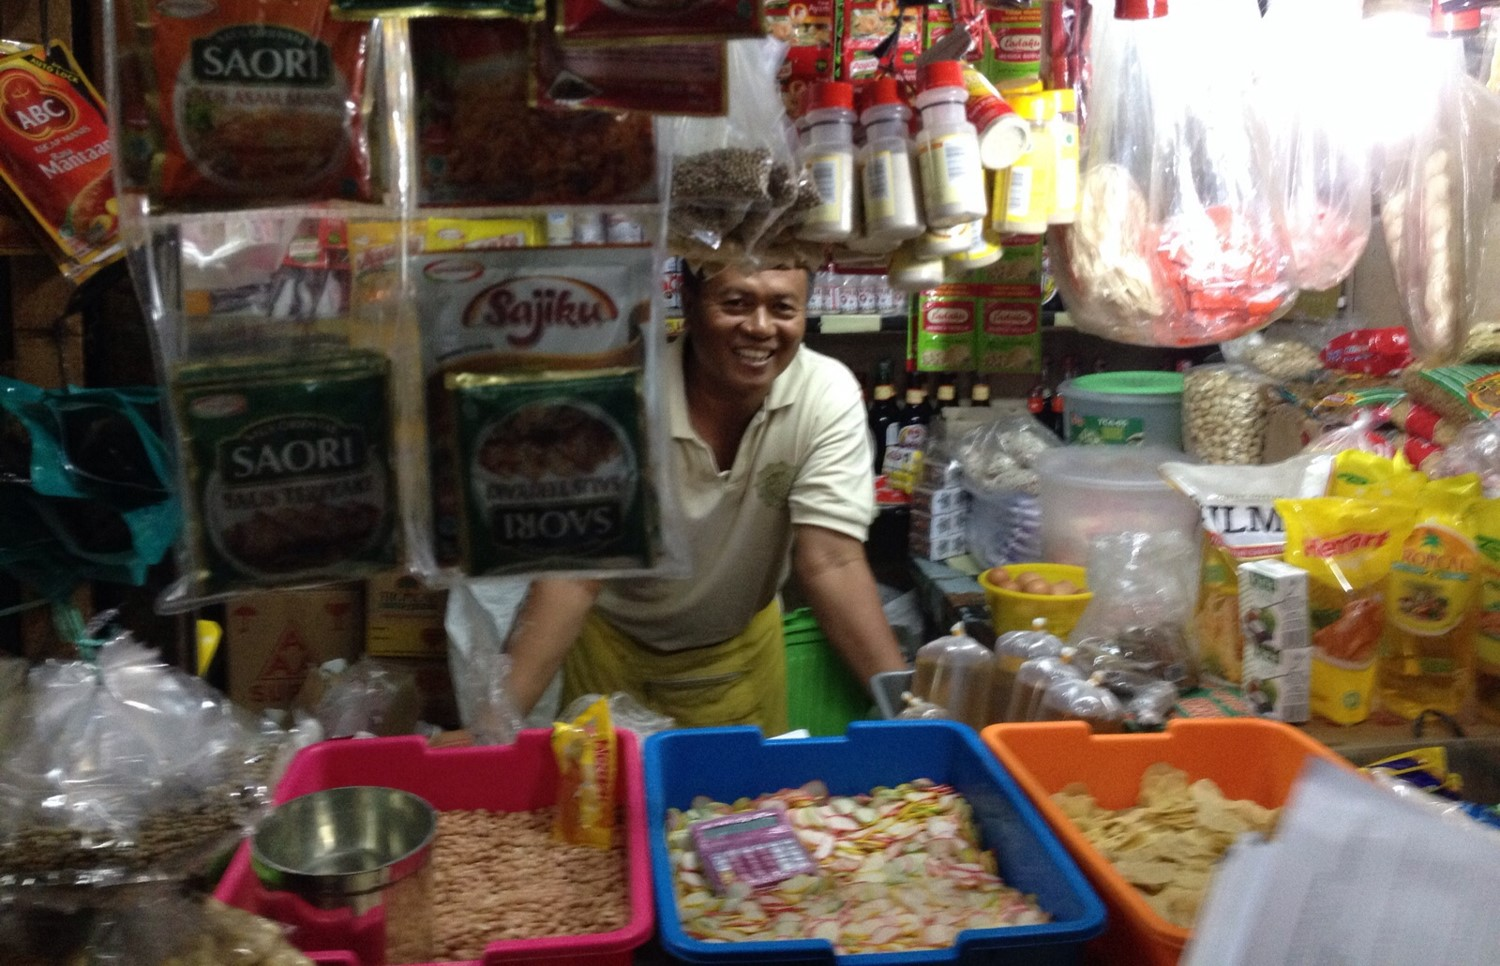
\includegraphics[width=4in]{pics/retailer1.jpg}
	%\caption{Best-practices handbook}
	\label{height}
\end{figure}
\end{frame}

\begin{frame}
\frametitle{Typical Business in the Sample}

\begin{figure}[htbp]
	\centering
		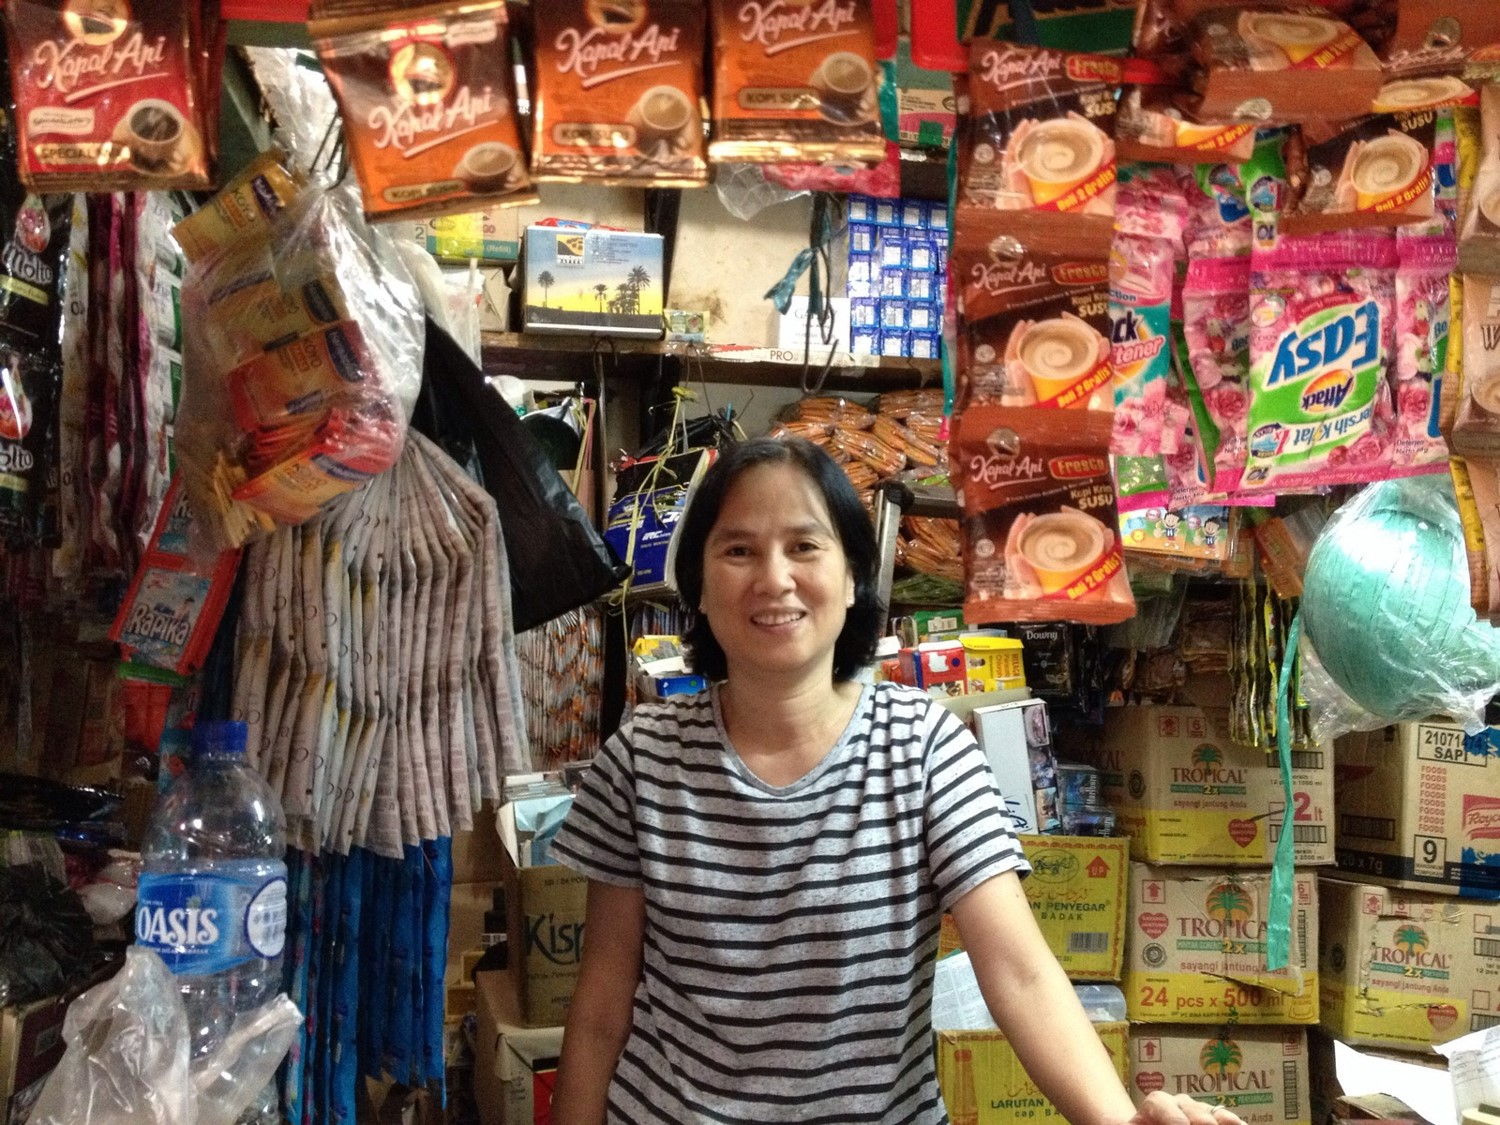
\includegraphics[width=4in]{pics/retailer2.jpg}
	%\caption{Best-practices handbook}
	\label{height}
\end{figure}
\end{frame}


\begin{frame}
\frametitle{Best-practices Handbook}

\begin{figure}[htbp]
	\centering
		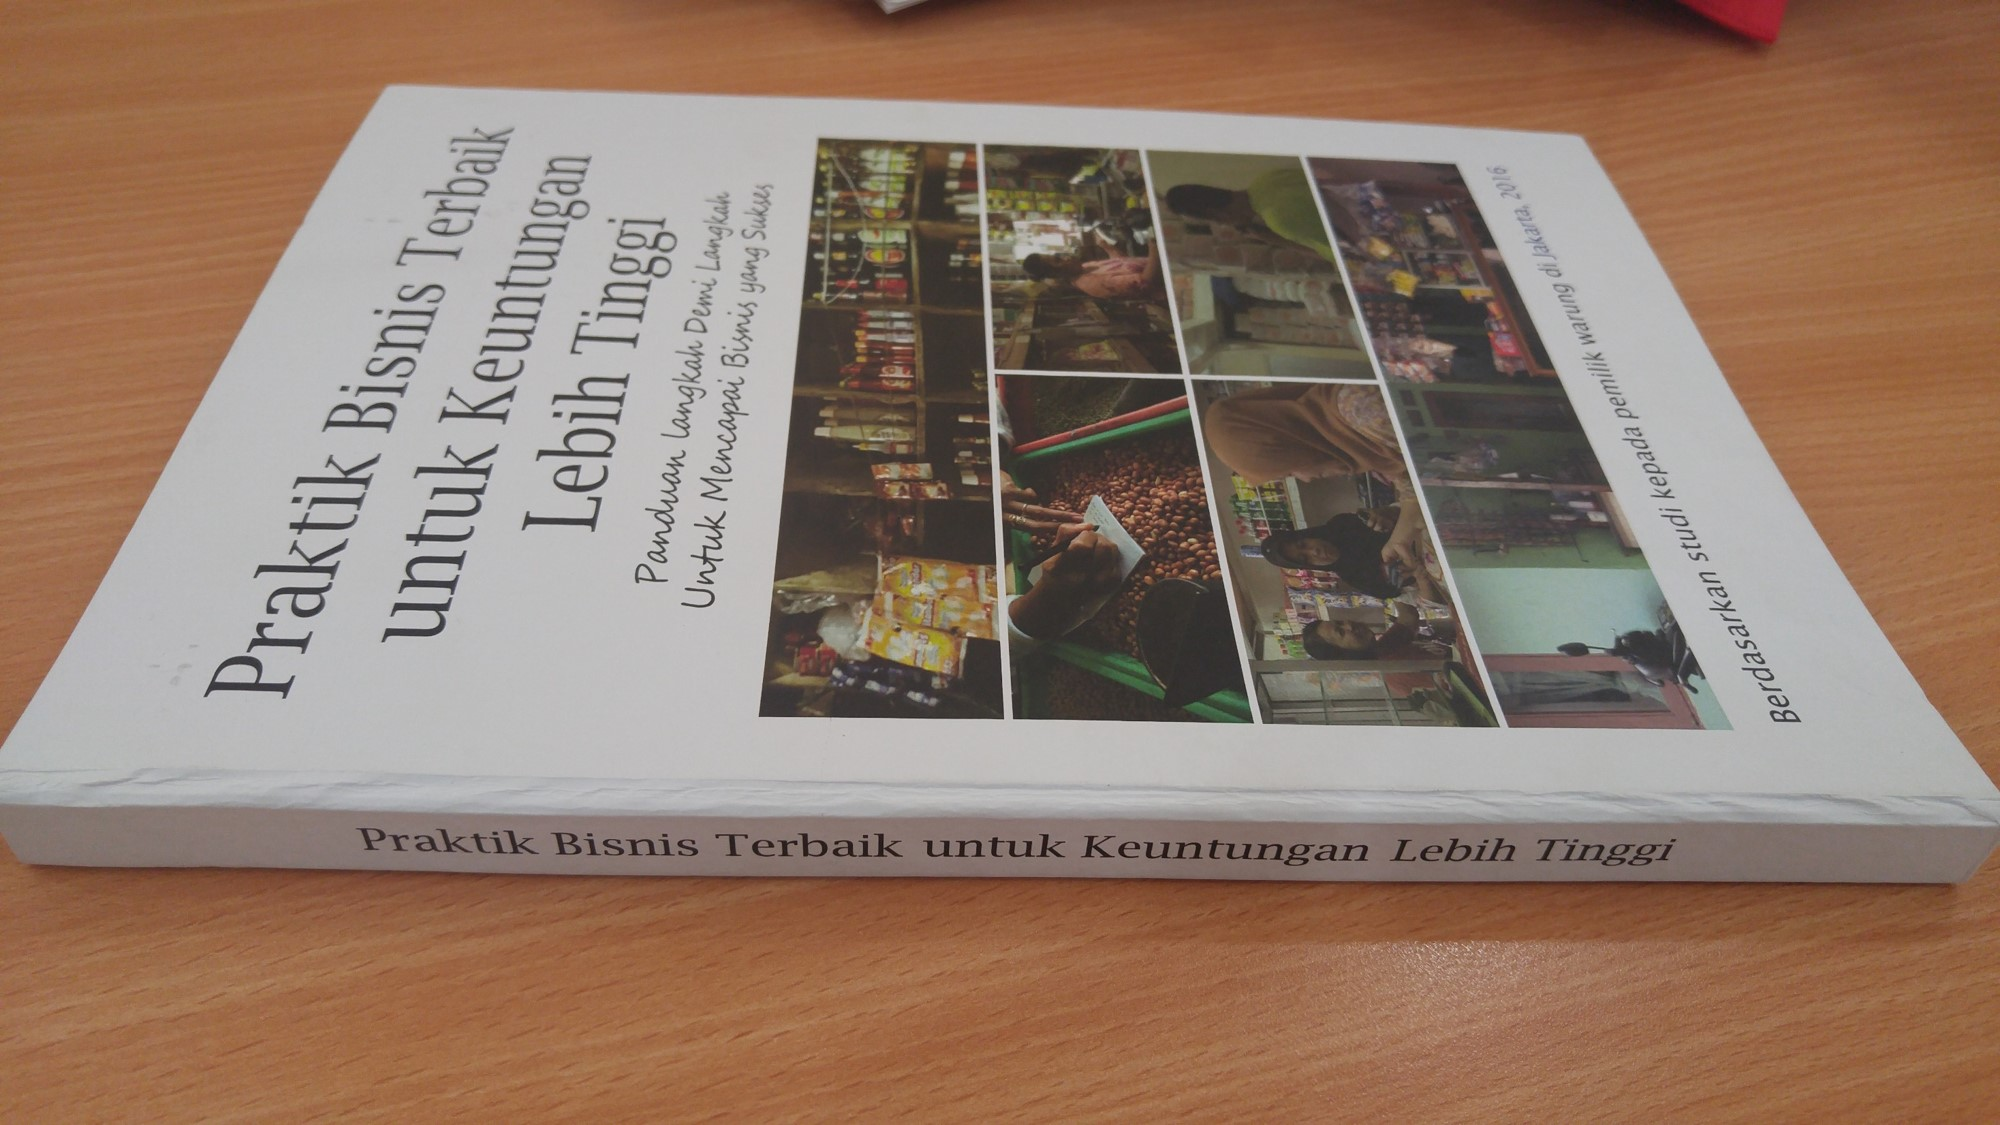
\includegraphics[width=4in]{pics/handbook.jpg}
	
	\label{height}
\end{figure}
\end{frame}


\begin{frame}
\frametitle{Handbook Content}
\begin{figure}[htbp]
	\centering
		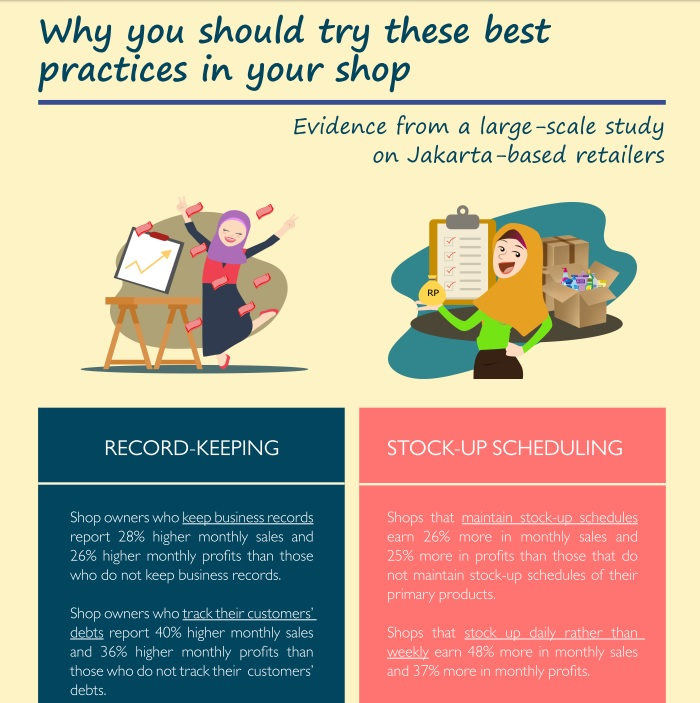
\includegraphics[width=2.6in]{pics/Handbook_return.jpg}
	
	\label{height}
\end{figure}
\end{frame}


\begin{frame}
\frametitle{Handbook Content}

\begin{figure}[htbp]
	\centering
		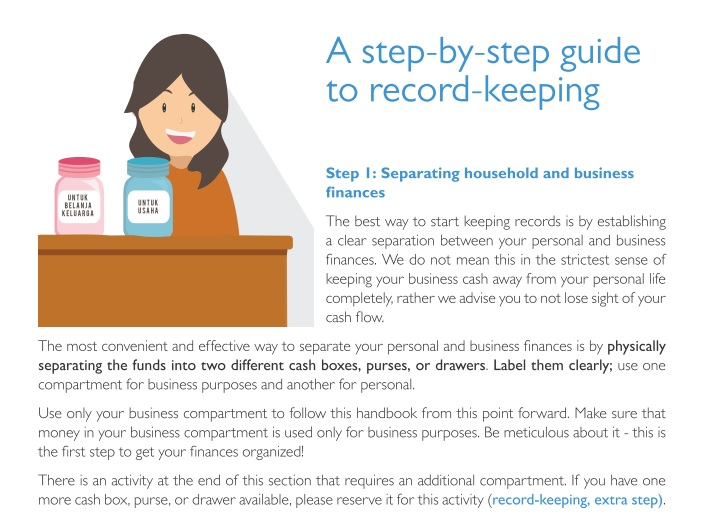
\includegraphics[width=2.6in]{pics/Handbook_stepbystep.jpg}
	
	\label{height}
\end{figure}
\end{frame}

\begin{frame}
\frametitle{Movie with Successful Peers}
\begin{figure}[htbp]
	\centering
		\includegraphics[width=4.4in]{pics/movie.jpg}
   
	\label{height}
\end{figure}
\end{frame}


\begin{frame}
\frametitle{Implementation Assistance for Business Practices}
\begin{figure}[htbp]
	\centering
		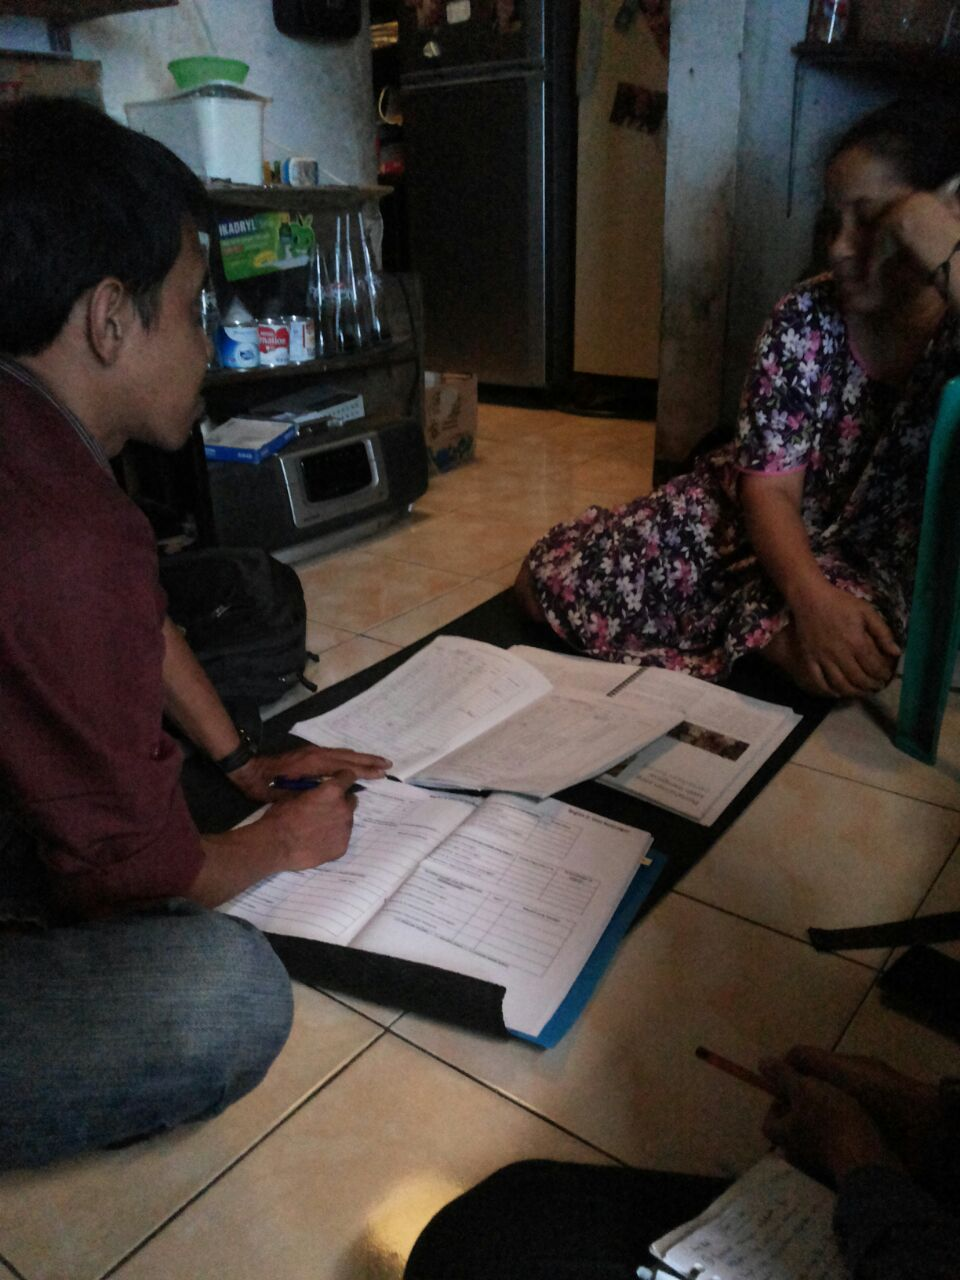
\includegraphics[width=2.0in]{pics/Assistance_expl.jpg}
	
	\label{height}
\end{figure}
\end{frame}


\subsection{Results}

\begin{frame}
\frametitle{Summary Statistics}
{\tiny{
	\begin{table}
		%\begin{adjustbox}{width=9.6cm}
		\centering	
		%\tabcolsep=0.2cm

			\begin{tabular}{l*{10}{c}}
			\hline\hline
			\hline


&\multicolumn{1}{c}{\textcolor{bdf}{Control}}
&&\multicolumn{1}{c}{\textcolor{bdf}{HB only}}	
&&\multicolumn{1}{c}{\textcolor{bdf}{HB \& MOV}	}
&&\multicolumn{1}{c}{\textcolor{bdf}{HB \& HELP}}	
&&\multicolumn{1}{c}{\textcolor{bdf}{HB \& MOV}}	\\


&\multicolumn{1}{c}{}
&&\multicolumn{1}{c}{}	
&&\multicolumn{1}{c}{}
&&\multicolumn{1}{c}{}	
&&\multicolumn{1}{c}{\textcolor{bdf}{\& HELP}}	\\


&\textit{N = 261}	
&&\textit{N = 260}	
&&\textit{N = 260}	
&&\textit{N = 260}	
&&\textit{N = 260}	\\
\hline \\

\textcolor{bdf}{Firm Owner Characteristics} \\
Gender (Male=1)											& 0.28	&& 0.3	&&0.29	&& 0.3	&& 0.28\\
Age														&45.22	&&45.27	&&45.28	&&45.16	&&45.38 \\
Education (Years)										&9.1	&&9.52	&&9.36	&&9.42	&&9.55 \\
%Digitspan												& 1.7	&& 1.67 && 	1.8 &&	1.67	&& 1.69 \\
														%&(1.12) 	&& 		&& 		&& 		&& 		&& \\
Risk Preference (0 - 10 ``Perfectly Risk-Seeking'')		&3.74	&&3.76	&&3.88	&&3.6	&&3.68 \\											
Time Preference	(0 - 10 ``Perfect Patience'')			&5.19	&&5.07	&&5.21	&&5.25	&&5.2 \\[0.5ex]
\\														
\textcolor{bdf}{Firm Characteristics} \\
Firm Age (Years)										&12.76		&&13.77		&&14.03		&&13.98		&&13.47 \\
Family Member Is Business Partner							&0.56		&&0.6		&&0.63		&&0.59		&&0.62 \\
Total Number of Workers									&2.03		&&2.05		&&1.9		&&1.99		&&2.04 \\
%Number of Full Time Paid Employees						&0.09		&&0.1		&&0.08		&&0.08		&&0.11		&&0.08 \\
														%&(0.3)		&&			&&			&&			&&			&& \\
Business Has Tax ID										&0.2		&&0.21		&&0.2		&&0.15		&&0.18 \\
Total Sales Last Month (USD PPP)						&4454.37 &&	4730.64	&& 4840.55	&& 4761.4	&& 5139 \\
												
Total Profits Last Month (USD PPP)						& 889.58	&& 961.1 &&	926.78	&& 825.25	&& 934.66 \\
Applied for Bus Loan in Last 12 Months
			    & 0.2	&& 0.17	&& 0.15	&& 0.22	&& 0.17 \\
													
Obtained Bus Loan in Last 12 Months
						& 0.18 &&	0.15	&& 0.14	&& 0.18	&& 0.14 \\[0.5ex]
\\
\\
\textcolor{bdf}{Business Practices} \\
Management Practices Aggregate Score											& 0.37	&& 0.36	&& 0.37	&& 0.35	&& 0.37 \\
\hspace{3mm}Marketing Subscore												& 0.23	&& 0.23 &&	0.25	&& 0.23	&& 0.24 \\
\hspace{3mm}Stocking-up	Subscore											& 0.45	&& 0.47	&& 0.47	&& 0.47	&& 0.46 \\
\hspace{3mm}Record-keeping Subscore											& 0.33	&& 0.28	&& 0.3	&& 0.29 &&	0.3 \\
\hspace{3mm}Financial-planning Subscore									& 0.51	&& 0.47	&& 0.47	&& 0.43	&& 0.47 \\
%\hspace{3mm} Discussion Subscore                        & 0.57	&& 0.59	  && 0.61	&& 0.6	&& 0.64  \\
&		&&		&&		&& \\
		\hline
		\hline
			\end{tabular}
		%\end{adjustbox}			
		
		%\begin{adjustbox}{center}
			%\begin{tabular}{l*{12}{l}}
			%\multicolumn{13}{p{0.95\textwidth}}{\footnotesize \textit{Notes}: $^1$ Last month's sales and profits appear with both tails winsorized at 1%.}
			%\end{tabular}
		%\end{adjustbox}	
		
	\end{table}}}
\begin{itemize_3pt}
\item Test of Joint Orthoganality from Multinomial Logit (P-value): 0.857
\end{itemize_3pt}
\end{frame}


\begin{frame}
\frametitle{Movie: Take Up and Assessment}
{\scriptsize{\begin{table}[htbp]
%\fontsize{10}{11}\selectfont
  \centering
 %   \tabcolsep=0.10cm
    %\begin{adjustbox}{width=11cm}
    \begin{tabular}{lcc}
    \hline
   	& (1)   					&(2)   						 \\
    \hline
  	& \textcolor{bdf}{HB \& MOV} 		& \textcolor{bdf}{HB \& MOV}		  \\
  	& 							& \textcolor{bdf}{\& HELP}			\\
   	& \textcolor{bdf}{(A)}   			& \textcolor{bdf}{(B)}   			 \\
 	&							&							\\
% 	&							&							&& \textit{F-test}\\
   	%	& Assigned 				& Assigned 					&&  \\
   	& \textit{N=260} 			& \textit{N=260} 			 \\
   \hline
   														&		&		 \\
    \textcolor{bdf}{Attendance} 								&       &         \\
  	% 													&		&		&& \\
    Business Owner or Partner Attended Film Screening 	& 0.52  & 0.49   \\
    %Baseline respondent attended film screening 		& 0.47  & 0.45  && 0.792 \\
   	%Respondent was reminded by phone 					& 0.05  & 0.07  && 0.355 \\
    %Respondent was reminded by visit to business 		& 0.35  & 0.33  && 0.782 \\
    %Distance to screening location (in decimal degrees)& 0.01  & 0.01  && 0.869 \\
	&       &       \\
    \textcolor{bdf}{Evaluation (1-4 Scale):}	&       &        \\
   	%									&       &       &&  \\
    Has Learned Something New	& 3.34  & 3.21  \\
    Feels Inspired 				& 3.31  & 3.30   \\
    Feels Hopeful 				& 3.60  & 3.42   \\
    Feels Bored 				& 0.83  & 0.97    \\
    \end{tabular}
   % \end{adjustbox}

\end{table}}}

\end{frame}


%%% Attendance and feedback to assistance + comparison between experimental groups
\begin{frame}

\frametitle{Assistance: Take Up and Assessment}
{\scriptsize{\begin{table}[htbp]
%\fontsize{10}{11}\selectfont
  \centering
    %\tabcolsep=0.10cm
   % \begin{adjustbox}{width=11cm}
    \begin{tabular}{lcc}
    \hline
    & (1)   			& (2) 			\\
    \hline
   	& \textcolor{bdf}{HB \& HELP} 		& \textcolor{bdf}{HB \& MOV,}		 \\
  	& 							& \textcolor{bdf}{\& HELP}			 \\
   	& \textcolor{bdf}{(A)}   			& \textcolor{bdf}{(B)}   			\\
	&							&							 \\
% 	&							&							&& \textit{F-test}\\
   	%	&& Assigned 				& Assigned 					&&  \\
   	& \textit{N=260} 			& \textit{N=260} 		\\
    \hline
          																				&       &      \\
    \multicolumn{1}{l}{\textcolor{bdf}{Attendance}} 											&       &        \\
    %\multicolumn{1}{l}{\textit{1st session}} 											&       &       & &  \\
    \multicolumn{1}{l}{    Business Owner or Partner Attended 1st Session} 				& 0.77  & 0.78  \\
    %\multicolumn{1}{l}{    Baseline respondent attended 1st session} 					& 0.76  & 0.77  && 0.756 \\
    %\multicolumn{1}{l}{    Recipient plans to use at least one new practice} 			& 0.37  & 0.47  && 0.021** \\
    %\multicolumn{1}{l}{    Recipient plans neither handbook study nor implementation} 	& 0.12  & 0.11  && 0.784 \\
         														 						%&     	&       &&  \\
    %\multicolumn{1}{l}{\textit{2nd session}} 											&       &       &&  \\
    \multicolumn{1}{l}{    Business Owner or Partner Attended 2nd Session} 				& 0.68  & 0.68   \\
    %\multicolumn{1}{l}{    Baseline respondent attended 2nd session} 					& 0.67  & 0.67  && 1 \\
    %\multicolumn{1}{l}{    Recipient plans to use at least one new practice} 			& 0.39  & 0.47  && 0.063* \\
    %\multicolumn{1}{l}{    Recipient plans neither handbook study nor implementation} 	& 0.13  & 0.08  && 0.044** \\
          																				&       &        \\
    \multicolumn{1}{l}{\textcolor{bdf}{Evaluation (1-4 Scale)}} 								&       &         \\
    \multicolumn{1}{l}{Has Learned Something New} 										& 2.88  & 2.89   \\
    \multicolumn{1}{l}{Feels Inspired} 													& 2.76  & 2.83   \\
    \multicolumn{1}{l}{Feels Hopeful} 													& 2.88  & 2.97  \\
    \multicolumn{1}{l}{Feels Bored} 													& 0.59  & 0.43   \\
    \end{tabular}
   % \end{adjustbox}

\end{table}}}
\end{frame}


\begin{frame}
\frametitle{Impact on Business Practices}
\framesubtitle{Aggregate Scores}
{\tiny{\begin{table}[t]
%\centering
%\begin{adjustbox}{width=10cm}
%	\tabcolsep=0.05cm
	\begin{tabular}{l*{10}{c}}
		\hline \hline
		\\
			&\textcolor{bdf}{Record}			&&\textcolor{bdf}{Planning}			&&\textcolor{bdf}{Stocking-up}	&&\textcolor{bdf}{Marketing} && \textcolor{bdf}{Joint} \\
&\textcolor{bdf}{Keeping}                       &&                        &&	                   &&	 && Decision-making \\
					&(1)					&&(2)						&&(3) 						&&(4) && (5)\\
			\cline{2-2}					\cline{4-4}					\cline{6-6}			\cline{8-8} \cline{10-10}  \\


Assigned Handbook 			&                    0.025   &&	          0.027   	 &&           -0.007   	 &&          -0.011   	  &&         0.011
      \\
         							&               (0.209)   	   &&      (0.273)   	&&         (0.694)   	     &&    (0.694)   	&&         (0.694)
    \\

         							
Assigned Handbook \& Movie 	&                     0.057*** 	 &&          0.043  	   &&       0.038  	    &&       0.040    &&        0.040        \\
          							&              (0.009)   &&	         (0.107)   	  &&       (0.117)   	  &&       (0.166)   	 &&        (0.217)         \\

         							
Assigned Handbook \& Assistance 	&              0.065*** 	  &&         0.034   	&&           0.011   	 &&           0.039 	       &&      0.037    \\
         							&           (0.004)   	  &&       (0.166)   &&	         (0.664)   && 	         (0.166)   	  &&       (0.239)    \\

         							
Assigned All Three          	&                0.054***	  &&         0.068***  	 &&          0.053**  	    &&       0.061**	   &&        0.059*          \\
									&             (0.009)    &&	         (0.009)   	&&         (0.020)   	  &&       (0.032)   &&	         (0.094)           \\

\hline         							
\\
R-squared									&               0.204   	 &&          0.192   	&&           0.187   	&&           0.150	 &&           0.120             \\
Sample Size 								&               2205   	  &&          2204   	   &&         2205   	 &&           2205   	    &&        2205      \\
Dependent Variable Mean of Control 		&                  0.196  	  &&         0.402   	 &&          0.471    &&	           0.250    	 &&          0.269          \\
Dependent Variable SD of Control 			&              0.252    	 &&          0.310   	  &&         0.270      	  &&         0.320    && 	           0.420        	\\
F-tests (p-value):							&			&&			&&			&&			\\
\hspace{5mm}Book = Book \& Mov				        &               0.069   	   &&           0.487   	  &&          0.014     	  &&          0.028    	 &&          0.300           \\
\hspace{5mm}Book = Book \& Assistance				        &               0.025  	  &&          0.754     	 &&           0.304   	 &&          0.030    	  &&          0.348                 \\
\hspace{5mm}Book = All Three				        &                  0.096    	  &&         0.073    	    &&      0.001   	  &&         0.002    &&	         0.082        \\
\hline
	\end{tabular}
%\end{adjustbox}
\end{table}}}
\begin{itemize_3pt}
\item Multiple hypothesis testing corrected p-values in parentheses
\item "All Three" improvement of 28 \% in record-keeping, 17 \% in planning, 11 \% in stocking, 24 \% in marketing and 22 \% in joint decision making.
\end{itemize_3pt}
\end{frame}


\begin{frame}

\frametitle{\centering{Business Profits}}
{\scriptsize{\begin{table}[t]
\centering
%\begin{adjustbox}{width=9cm}
%	\tabcolsep=0.05cm
	\begin{tabular}{l*{5}{c}}
\hline
\hline
			   &&Profits	        &&Profits \\
				&&last month  		&&last month \\
			&&(win 5\%)			&&(IHS) \\
				&&(1)				&&(2)	\\
&& \\
					\hline
&&\\
		

Assigned Handbook 					&&-91.307   	&& -0.067   		\\
       								 	&&         (78.400)  	&&          (0.088)  	\\

         							
Assigned Handbook \& Movie				&&110.378   	  	&& 0.055   		\\
       									&&         (86.841)  	&&          (0.092)  	\\

         							
Assigned Handbook \& Assistance 	&&         310.455***	&&           0.261***		\\
       								 	&&         (89.488) 	&&          (0.096)  	\\
         							
Assigned All Three          		&&         191.088**  	&&           0.199** 		\\
       								 	&&         (84.662)  	&&          (0.094)  	\\

   	\\
\hline         							
\\
R-squared											  	&& 0.179  	&& 0.211  	\\
Sample Size 											&&2172	&& 2172 	\\
Dependent Variable Mean in Control Group			 	&&          894.544   	&&           6.817 	\\
Dependent Variable SD in Control Group				 	&&         1127.783   	 &&          1.348  	\\
F-tests (p-value):											&&			&&			\\
\hspace{5mm}Book = Book \& Mov				        	&&    0.020   	&&            0.167 	\\
\hspace{5mm}Book = Book \& Assistance				  			&&0.000   	&&0.000  	\\
\hspace{5mm}Book = All Three			   			  	&&0.001   	&&0.003  	\\
\hline
	\end{tabular}
%\end{adjustbox}

\end{table}}}
\begin{itemize_3pt}
\item Profits increase by 35\% (about 0.28 sd.) - ITT.
\end{itemize_3pt}
\end{frame}




\begin{frame}
\frametitle{Business Sales}
{\scriptsize{\begin{table}[t]
\centering
%\begin{adjustbox}{width=9cm}
%	\tabcolsep=0.05cm
	\begin{tabular}{l*{5}{c}}
\hline
\hline
                &&ITT	        &&TOT \\
			   &&Sales	        &&Sales \\
				&&last month  		&&last month \\
			&&(win 5\%)			&&(win 5\% \\
				&&(1)				&&(2)	\\
&& \\
					\hline
&&\\
		

Assigned Handbook 					&&-396.976   	&&               -417.198		\\
       								 	&&        (314.252)   	&&          -417.198	\\

         							
Assigned Handbook \& Movie				&&335.489   	  	&& 601.221    		\\
       									&&       (337.881)  	&&            (606.634)	\\

         							
Assigned Handbook \& Assistance 	&&                   836.755**	&&                     1031.692** 	\\
       								 	&&        (372.924) 	&&            (457.015) 	\\
         							
Assigned All Three         		&&         807.462**  	&&                         1558.326**		\\
       								 	&&        (358.384)  	&&          (696.317)   	\\

   	\\
\hline         							
\\
R-squared											  	&& 0.492  	&&  0.483	\\
Sample Size 											&& 2197	&& 2197 	\\
Dependent Variable Mean in Control Group			 	&&         4998.923   &&	          4998.923 	\\
Dependent Variable SD in Control Group				 	&&         5623.257   	&&           5623.257	\\
F-tests (p-value):											&&			&&			\\
\hspace{5mm}Book = Book \& Mov				        	&&            0.020 	&&           0.047 	\\
\hspace{5mm}Book = Book \& Assistance				  			&&0.000   	&& 0.000 	\\
\hspace{5mm}Book = All Three			   			  	&&0.000   	&&0.001  	\\
\hline
	\end{tabular}
%\end{adjustbox}

\end{table}}}
\begin{itemize_3pt}
\item Sales increase by 16\% (about 0.15 sd.) - ITT %- and 31\% (0.28 sd.) - TOT.
\end{itemize_3pt}
\end{frame}


\begin{frame}
\frametitle{Other Outcomes}
\begin{itemize_3pt}
\item \textcolor{bdf}{No significant} impacts on:
    \begin{itemize_3pt}
    \vspace{0.1in}
    \item Business expenses
    \vspace{0.1in} 		
    \item Size of the shop
      \vspace{0.1in}
    \item Number of employees
      \vspace{0.1in}
    \item Number of customers
       \vspace{0.1in}
     \item Business credit
    \end{itemize_3pt}
\end{itemize_3pt}
\end{frame}

\subsection{Discussion}
\begin{frame}
\frametitle{Efficiency Gains?}
\begin{enumerate_3pt}
\item Unpacking impacts on practices shows improvements in efficiency practices:
\vspace{0.1in}
\begin{itemize_3pt}
\item Adjust stocks based on product profitability
\item Negotiate lower prices with suppliers
\item Consult with former customers
\item Offer discounts
\item Make joint decisions
\item Review financial performance to identify channels of improvement
\item Make anticipated budget for upcoming costs
\end{itemize_3pt}
\vspace{0.1in}
\pause
\item These are non-record-keeping practices. Also, variance in profits among the treated businesses does not converge
\vspace{0.1in}
\pause
\item Causal-mediation analysis shows that the most important drivers of impact on sales and profits are stocking up and marketing practices.
\end{enumerate_3pt}
\vspace{0.1in}
$\rightarrow$ \textcolor{bdf}{Efficiency gains}
\end{frame}

\begin{frame}
\frametitle{Knowledge or Aspirations?}
\begin{itemize_3pt}
\item Our interventions could have increased business performance and practice adoption through an increase in business aspirations rather than (or on top of) business knowledge.
\vspace{0.1in}
\item We directly measure business aspirations at baseline, midline, and endline for all shop owners in the sample.
\vspace{0.1in}
\item We elicit short (one year) and long-term (ideal) aspirations on various business dimensions:
\vspace{0.1in}
    \begin{itemize_3pt}
    \item sales
    \item shop size
    \item number of customers
    \item number of employees
    \end{itemize_3pt}
\vspace{0.1in}
\item No treatment effects on aspirations
\vspace{0.1in}
\end{itemize_3pt}
$\rightarrow$ \textcolor{bdf}{Knowledge}
\end{frame}

\begin{frame}
\frametitle{Business Stealing?}
Do treated businesses improve performance at the expense of the control?
\vspace{0.1in}
\begin{itemize_3pt}
\item Sales and profits of \textcolor{bdf}{control businesses do not decrease} from baseline to endline (roughly equal)
\item Sales and profits of control businesses \textcolor{bdf}{closer to treated shops do not decrease by more} than those further away
\item[] $\rightarrow$ \textcolor{bdf}{No evidence for business stealing}
\end{itemize_3pt}
\end{frame}

\begin{frame}
\frametitle{Cost-Effectiveness}

\textcolor{bdf}{Small costs (per firm)}:
\begin{itemize_3pt}
\item Cost Handbook alone: USD 100
\item Cost Handbook \& Movie: USD 125
\item Cost Handbook \& Assistance: USD 125
\item Cost Handbook \& Movie \& Assistance: USD 150
\end{itemize_3pt}
\vspace{0.5em}

\textcolor{bdf}{Substantial Benefits}
\begin{itemize_3pt}
\item Up to USD 330 per month in profits
\item Adoption of top practices by retailers
\end{itemize_3pt}

\vspace{0.5em}
Research design likely \textcolor{bdf}{scalable and portable}

\end{frame}

\subsection{Conclusion}
\begin{frame}
\frametitle{Takeaways}
\begin{itemize_3pt}
    \item \textcolor{bdf}{Curating local knowledge has value for business growth} 
    \item Information alone does not have impact, only combined with \textcolor{bdf}{behavioral interventions}
    \item Mechanism likely \textcolor{bdf}{knowledge-based}, not aspirations-based
	\item Behavioral interventions are \textcolor{bdf}{inexpensive and scalable}
	\vspace{-0.5em}
	\item[] $\rightarrow$  Attractive for policy!
    
\end{itemize_3pt}
\end{frame}


%\bibliographystyle{econometrica}
%\bibliography{sampleBibFile}


\end{document}
